\chapter{\IfLanguageName{dutch}{Stand van zaken}{State of the art}}%
\label{ch:stand-van-zaken}

% Tip: Begin elk hoofdstuk met een paragraaf inleiding die beschrijft hoe
% dit hoofdstuk past binnen het geheel van de bachelorproef. Geef in het
% bijzonder aan wat de link is met het vorige en volgende hoofdstuk.

% Pas na deze inleidende paragraaf komt de eerste sectiehoofding.


In de afgelopen jaren zijn er heel wat nieuwe JavaScript runtime-omgevingen geïntroduceerd. Echter worden weinig van deze omgevingen effectief gebruikt.
Zo toont het eerder vermelde onderzoek van \textcite{Greif2022} aan dat Node.js nog steeds als standaard gebruikt wordt bij de meeste projecten 
ondanks de tal van nieuwe runtime-omgevingen.
In dit onderzoek wordt nagegaan of één van deze nieuwe frameworks
een correcte plaatsvervanger kan zijn voor Node.js bij de ontwikkeling van webapplicaties waar performantie centraal staat.
Daarom wordt er dieper ingegaan op deze technologieën om zo een beter inzicht te krijgen in het onderzoeksdomein.
Ten eerste wordt een precieze beschrijving gegeven over de programmeertaal JavaScript en hoe deze wordt gebruikt bij de runtime-omgevingen.
Hierbij wordt de architectuur van een JavaScript runtime-omgeving beschreven.
Nadien wordt verder ingegaan op 3 van deze omgevingen namelijk Node.js, Deno en Bun. 
Hierbij wordt gekeken naar hun respectievelijke JavaScript engine, package managers, bundlers en functionaliteiten.
Als laatste wordt gekeken naar eerder onderzoek over deze onderwerpen. 
Hierbij wordt verder ingegaan op de performantie metrieken die kunnen gebruikt worden alsook de bijhorende 
software om deze te achterhalen.

\section{JavaScript}
JavaScript is een programmeertaal die gebruikt wordt om applicaties te ontwikkelen. 
Specifiek is het een scripting taal die web pagina's interactief kan maken~\autocite{Mozilla2023}.
Hierbij spreken we over client-side JavaScript. Wanneer een web pagina wordt bekeken zal de JavaScript code worden 
gedownload en uitgevoerd~\autocite{JonathanBrownCFA2024}. Aan de andere kant heb je ook nog Server-side JavaScript. 
Hierbij wordt de code uitgevoerd op de server in plaats van op de client~\autocite{JonathanBrownCFA2024}. 
Voor deze code dan te laten uitvoeren is een JavaScript runtime-omgeving nodig. 

\subsection{JavaScript runtime-omgeving}
Een JavaScript-omgeving bestaat uit alle componenten om JavaScript correct te laten werken ~\autocite{Christopher}. 
Het bevat een JavaScript engine, WEB APIs en een callback queue ~\autocite{Christopher}. 
Deze runtime zal dan JavaScript code omzetten in code die verstaanbaar is voor de computer.
De omgeving specificeert waar dit wordt gedaan, dit kan in een browser maar ook in andere omgevingen zoals een server.
Met behulp van JavaScript runtime-omgevingen zoals Node.js en Bun kan JavaScript code ook buiten de browser worden uitgevoerd~\autocite{Mozilla2023}.

\subsubsection{JavaScript engine, WEB APIs en callback queue}

In een artikel van ~\textcite{Christopher}, 
wordt uitgelegd dat de JavaScript engine een simpel computer programma is dat de code kan interpreteren en uitvoeren.
Elk browser heeft achterliggend zijn eigen JavaScript engine. Het meest bekende hiervan is de
V8 engine die zowel bij Google chrome als Node.js wordt gebruikt. 
Wanneer een stuk code in de engine wordt ingevoerd,zal deze eerst geanalyseerd worden (parsing). 
De code wordt hierbij omgezet in een data structuur genaamd de abstract syntax tree (AST).
Wanneer deze boom is aangemaakt zal de compiler deze omzetten naar machine code. 
Eenmaal deze code is gegenereerd zal de engine zogenaamde execution contexts aanmaken om de code uit te voeren.
In figuur ~\ref{fig:JavaScriptengine} wordt hiervan een visuele voorstelling getoond.
\begin{figure}[H]
    \centering
    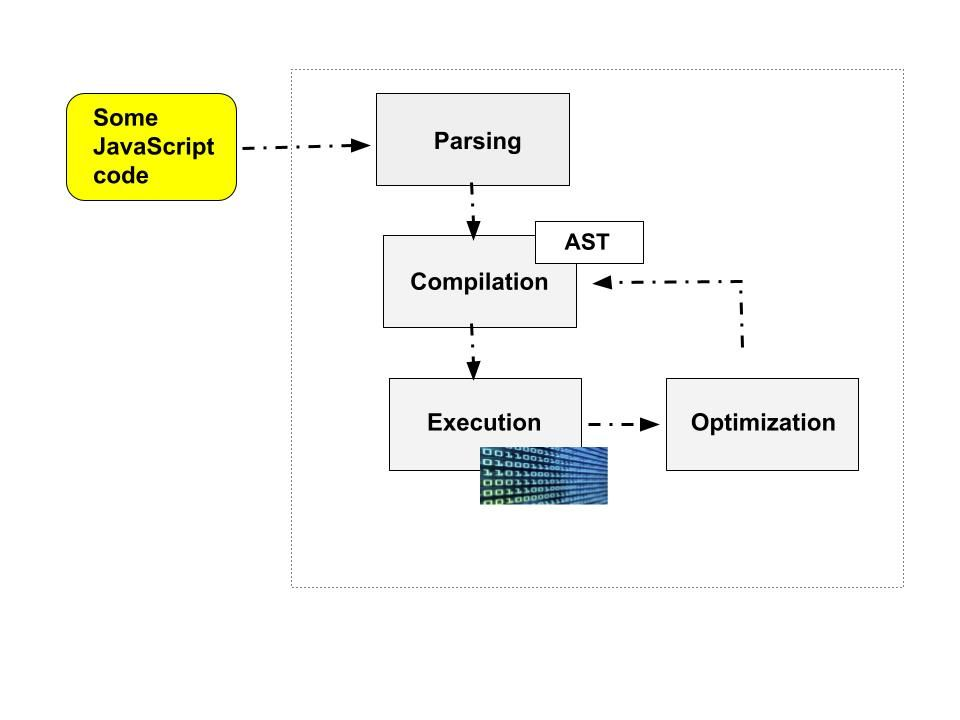
\includegraphics[width=.9\textwidth]{graphics/javascriptengine.jpeg}
    \caption[Werking JavaScript engine]{\label{fig:JavaScriptengine}Visuele voorstelling van werking JavaScript engine ~\autocite{Christopher}}
\end{figure}

Naast een JavaScript engine bevat een runtime-omgeving ook WEB APIs en een callback queue. 
WEB APIs zijn functionaliteiten die specifiek voor de runtime omgeving zijn en dus geen deel uitmaken van de JavaScript taal.
Voorbeelden hiervan zijn het manipuleren van documenten of het ophalen van data.
De callback queue bevat callback functies die volgens de First-In-First-Out methode worden uitgevoerd.
Dit zijn functies die als parameters aan andere functies kunnen worden doorgegeven en 
daarna binnen die functies kunnen worden opgeroepen ~\autocite{Eygi2020}.

\subsection{JavaScript bundler}
In de meeste projecten worden er verschillende modules gemaakt met JavaScript code. 
Om te zorgen dat deze modules goed kunnen samenwerken wordt een bundler gebruikt. 
Zo legt ~\textcite{Laurila2020} in haar thesis uit dat sommige modules afhankelijk van elkaar kunnen zijn. 
Hierdoor moeten deze in de juiste volgorde worden uitgevoerd. Een bundler zal aan de hand van deze afhankelijkheden 
een afhankelijkheidsgrafiek maken om ze de modules in 1 of meerdere bestanden te bundelen. 
Na de transformatie van de modules worden er ook nog optimalisaties gedaan zoals het verwijderen van opmerkingen en witte ruimte.
Daarnaast zorgt het bundelen van modules ervoor dat er minder netwerkverzoeken gedaan moeten worden.

\section{Node.js}
De afgelopen jaren is het aantal runtime-omgevingen sterk toegenomen. De meest bekende en oudste hiervan is Node.js.
Node.js is een server-side framework dat wordt gebruikt voor schaalbare applicaties te maken ~\autocite{Gackenheimer2013}.
Het maakt gebruik van de V8 JavaScript engine ontwikkeld door Google en heeft zijn eigen package manager genaamd Node Package Manager (npm).
Node.js is hoofdzakelijk geschreven in de programmeertalen C en C++.

\subsection{Event loop}
In het boek van ~\textcite{Ali2013} wordt verteld hoe Node.js zich onderscheidt van andere platformen door het gebruik van een event loop.
Wanneer in Node.js data wordt gelezen of geschreven zal een gebeurtenis worden uitgezonden. 
Aan de hand van callbacks, verwijzingen naar uitvoerbare code, kan gereageerd worden op deze gebeurtenissen. 
Concreet zijn de callbacks functies die als argument worden meegegeven aan asynchrone functies ~\autocite{Kumar2023}. 
De event loop zal hierbij continu kijken of er gebeurtenissen voorkomen. Wanneer een gebeurtenis plaatsvindt, zullen de gegenereerde callbacks in de event wachtrij geplaatst worden.
Zodra de asynchrone operatie compleet is en de event loop de callback in de wachtrij bereikt, wordt deze daadwerkelijk uitgevoerd ~\autocite{Kumar2023}.
Hierdoor kan Node.js taken uitvoeren waarbij het niet moet wachten op de voltooiing van 1 taak om al aan een andere te beginnen. 
Dit laat toe om I/O operaties asynchroon te maken zonder hierbij multithreading te gebruiken.
In figuur ~\ref{fig:eventloop} wordt hiervan een visuele voorstelling getoond.
\begin{figure}[h]
    \centering
    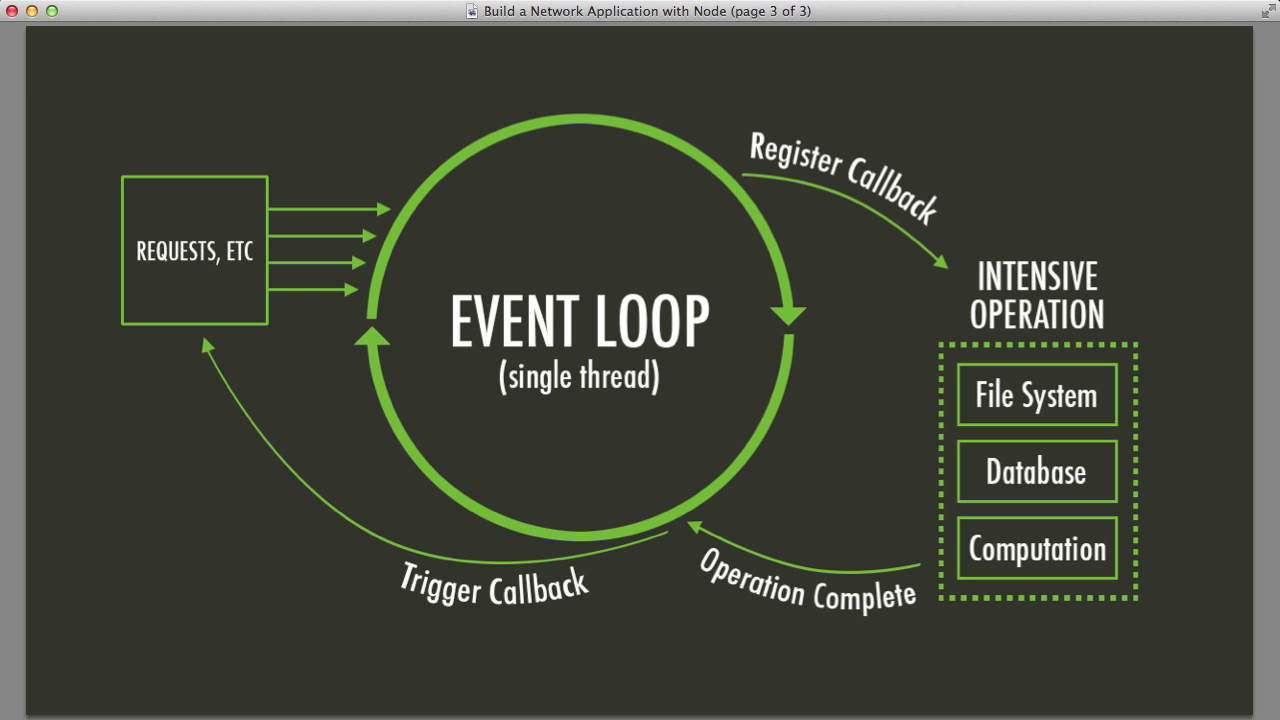
\includegraphics[width=.9\textwidth]{graphics/eventloop.png}
    \caption[Voorstelling event loop]{\label{fig:eventloop}Visuele voorstelling van de event loop ~\autocite{Luxembourg2023}}
\end{figure}

\subsection{Node Package Manager}
Node.js maakt gebruik van modules om code te hergebruiken. 
Zo vormt een module een stuk herbruikbare JavaScript code 
die je kan importeren in een ander JavaScript bestand ~\autocite{Semah2022}.
Naast deze zelf te maken kan je ook modules of packages van andere ontwikkelaars gebruiken met behulp van de Node Package Manager.
Veel van deze packages hangen af van nog andere packages om correct te werken \autocite{kula2017}.
Aan de hand van een package.json bestand kunnen packages toegevoegd worden aan een project.

\begin{listing}[H]
    \centering
    \begin{minted}[bgcolor=bg,
        fontfamily=tt,
        linenos=true,
        numberblanklines=true,
        numbersep=5pt,  
        gobble=0,
        framesep=2mm,
        tabsize=4,
        obeytabs=false,
        breaklines=true,
        mathescape=false
        samepage=false,
        showspaces=false,
        showtabs =false,
        texcl=false]{js}
        {
          "dependencies": {
            "foo": "1.0.0 - 2.9999.9999",
            "bar": ">=1.0.2 <2.1.2",
            "baz": ">1.0.2 <=2.3.4",
            "boo": "2.0.1",
            "qux": "<1.0.0 || >=2.3.1 <2.4.5 || >=2.5.2 <3.0.0",
            "asd": "http://asdf.com/asdf.tar.gz",
            "til": "~1.2",
            "elf": "~1.2.3",
            "two": "2.x",
            "thr": "3.3.x",
            "lat": "latest",
            "dyl": "file:../dyl"
            }
        }
        \end{minted}
        \caption[Voorbeeld package.json]{Voorbeeld package.json \autocite{Kaplan2024}}
\end{listing}

\subsection{V8 JavaScript Engine}
Zoals hierboven werd uitgelegd bestaat elk JavaScript runtime-omgeving uit een JavaScript engine die de code kan interpreteren en uitvoeren.
Node.js gebruikt hiervoor de V8 JavaScript engine van Google en voegt hierbij extra functionaliteit toe zoals de event loop.
In een artikel van ~\textcite{Lyamkin2020} wordt uitgelegd hoe de V8 engine precies werkt. 
Zo zal wanneer een JavaScript bestand wordt uitgevoerd eerst de code moeten omgezet worden op een manier dat verstaanbaar is voor de compiler.
Dit proces heet parsing en houdt in dat de code wordt omgezet in een AST (Abstract Syntax Tree). 
Nadien wordt deze doorgegeven aan de compiler zodat het dit kan omzetten in machine code. 
In de meeste programmeertalen zoals Java en C++ wordt dit gedaan vóór de executie van het programma (compilatie).
Bij dynamisch getypeerde talen zoals JavaScript wordt dit echter tijdens de runtime gedaan (interpretatie). 
Dit omwille dat het onmogelijk is het exacte type te weten vóór de executie.
Interpretatie is vaak trager dan compilatie doordat het geen optimalisaties kan doen.
Om deze transformatie sneller te laten gebeuren wordt aan Just-In-Time compilatie gedaan.
Hierbij gebruikt de V8 JavaScript engine een interpreter genaamd Ignition. Deze neemt de AST en zal hieruit de byte code genereren.
Nadien worden tijdens de executie de instructies geïnterpreteerd aan de hand van een tabel die de handler functies bevat en gekoppeld 
is aan de byte code.
Hierbij wordt ook type feedback verzameld over de code. 
Wanneer een functie vaak wordt gebruikt zal het geoptimaliseerd worden in de Turbofan compiler.
Deze neemt de byte code en type feedback en gaat op basis daarvan geoptimaliseerde machine code produceren.
Hier bestaat echter de kans dat het type kan veranderen door de dynamische aard van JavaScript. 
Dan wordt de gecompileerde code gedeoptimaliseerd, waarna het opnieuw wordt geïnterpreteerd.
Nadien kan de functie opnieuw gecompileerd worden met de nieuwe type feedback.
In figuur ~\ref{fig:v8} wordt dit proces nog eens visueel voorgesteld.
\begin{figure}[h]
    \centering
    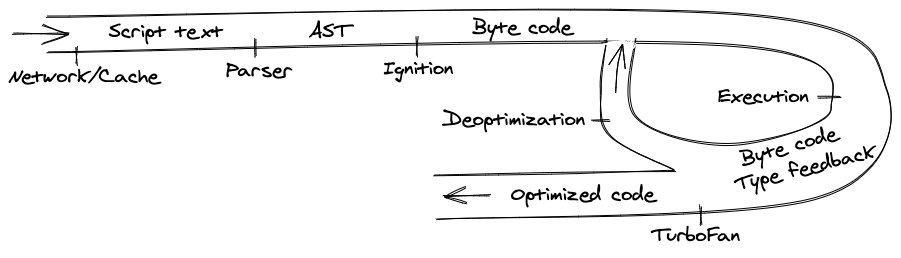
\includegraphics[width=.9\textwidth]{graphics/v8.png}
    \caption[Werking V8 engine]{\label{fig:v8}Visuele voorstelling van de werking van V8 ~\autocite{Lyamkin2020}}
\end{figure}

\subsection{Bundler}
Binnen Node.js zijn er verschillende mogelijkheden voor een bundler. De meest bekende hiervan is Webpack. 
Deze kan bestanden zoals JavaScript, SASS en andere bundelen naar hun respectievelijke bestandstype ~\autocite{Laurila2020}. 
Webpack kan daarnaast ook nog aangevuld worden met andere loaders om een bepaald soort bestand te bundelen ~\autocite{Laurila2020}. Een andere populaire bundler is Esbuild.
Hierbij wordt de focus gelegd op snelheid en performantie. Zo wordt er beweerd dat deze bundler 10 tot 100 keer sneller is dan de andere bundlers ~\autocite{Couriol2020}.
Het kan deze snelheid behalen doordat het geschreven is in de programmeertaal Go waarbij taken worden geparallelliseerd om zo gebruik te maken van meerkernige processors ~\autocite{Couriol2020}.

\section{Deno}
In 2021 werd een nieuw runtime-omgeving geïntroduceerd door ~\textcite{Dahl2021} genaamd Deno.
Dahl, de maker van Node.js, en Belder willen met Deno nieuw leven inblazen in het ecosysteem door middel van een
modern, productief programmeersysteem aan te bieden dat zich houdt aan browser APIs.

\subsection{Architectuur}
Net zoals Node.js gebruikt Deno onderliggende de V8 JavaScript engine ~\autocite{DenoLand2023}. 
Echter werd gekozen om Deno te ontwikkelen in Rust in plaats van C en C++ zoals bij Node.js ~\autocite{DenoLand2023}.
Een van de voornaamste doelen bij Deno is om de server side JavaScript dichter bij de browser JavaScript te krijgen.
Dit wordt bereikt door dezelfde APIs aan te bieden langs de server kant en de browser kant ~\autocite{Barrow2022}.

\subsection{Beveiliging}
Een belangrijk kenmerk van Deno is de standaard runtime-beveiliging.
Dit houdt in dat de code expliciet toegang moet geven tot gevoelige APIs zoals bestandssystemen, netwerken, enzovoort ~\autocite{DenoLand2023}. 
Hierbij wordt gebruikgemaakt van permissie vlaggen die toegang geven tot specifieke functionaliteiten zoals te zien is in ~\ref{fig:denocli}.

\begin{listing}[H]
    \centering
    \begin{minted}[bgcolor=bg,
        fontfamily=tt,
        linenos=true,
        numberblanklines=true,
        numbersep=5pt,  
        gobble=0,
        framesep=2mm,
        tabsize=4,
        obeytabs=false,
        breaklines=true,
        mathescape=false
        samepage=false,
        showspaces=false,
        showtabs =false,
        texcl=false]{shell}
        deno run --allow-net hello.ts
        \end{minted}
        \caption[Toelaten netwerk permissie]{\label{fig:denocli}Voorbeeld toelaten netwerk permissie met de --alow-net vlag \autocite{DenoLand2023}}
\end{listing}

\subsection{Package manager}
In tegenstelling tot Node.js komt Deno niet meegeleverd met een package manager. 
Het maakt echter gebruik van URLs om externe packages te importeren \autocite{DenoLand2023}.
Dit laat package developers toe om hun code te hosten waar ze zelf willen \autocite{Barrow2022}.
\textcite{Choubey2021} merkt echter op dat dit voor beschikbaarheidsproblemen kan zorgen. 
Terwijl er bij NPM een gegarandeerde beschikbaarheid was van de packages, is dit niet het geval bij Deno.
Een oplossing hiervoor is gebruik te maken van een apart bestand waarbij alle packages worden gedownload en gecachet op voorhand zoals in ~\ref{list:dept.ts}.
\begin{listing}[H]
    \centering
    \begin{minted}[bgcolor=bg,
        fontfamily=tt,
        linenos=true,
        numberblanklines=true,
        numbersep=5pt,
        gobble=0,
        framesep=2mm,
        tabsize=4,
        obeytabs=false,
        breaklines=true,
        mathescape=false
        samepage=false,
        showspaces=false,
        showtabs =false,
        texcl=false]{js}
//deps.ts
//directly from GitHub
export * as bodyParser from "https://raw.githubusercontent.com/mayankchoubey/deno-native-body-parser/v0.1.3/mod.ts";
//From Deno's standard library
export * as httpServer from "https://deno.land/std@0.96.0/http/server.ts";
//From Deno's third-party module service
export * as jwt from "https://deno.land/x/djwt@v2.2/mod.ts";
        \end{minted}
        \caption[Deno packages downloaden]{\label{list:dept.ts}Voorbeeld bestand waar alle packages worden gedownload en geexporteerd om te gebruiken binnen de applicatie  ~\autocite{Choubey2021}} 
\end{listing}

\subsection{Bundler}
Deno heeft een module genaamd 'emit' die een enkele JavaScript bundel kan genereren met dependencies ~\autocite{DenoLand2023a}. 
Echter is dit enkel bedoeld voor gebruik binnenin Deno zelf en niet binnenin andere runtimes. 
Hiervoor kunnen andere bundlers gebruikt worden, zoals die besproken bij Node.js.

\begin{listing}[H]
    \centering
    \begin{minted}[bgcolor=bg,
        fontfamily=tt,
        linenos=true,
        numberblanklines=true,
        numbersep=5pt,
        gobble=0,
        framesep=2mm,
        tabsize=4,
        obeytabs=false,
        breaklines=true,
        mathescape=false
        samepage=false,
        showspaces=false,
        showtabs =false,
        texcl=false]{js}
import { bundle } from "https://deno.land/x/emit/mod.ts";
const result = await bundle(
"https://deno.land/std@0.140.0/examples/chat/server.ts",
);

const { code } = result;
console.log(code);
        \end{minted}
        \caption[Bundling via emit module]{\label{list:bundle}Voorbeeld bundling via emit module  ~\autocite{DenoLand2023a}} 
\end{listing}
\subsection{TypeScript ondersteuning}
In tegenstelling tot Node.js ondersteunt Deno TypeScript als standaard. 
Deno zal TypeScript als een eerste klas taal behandelen wat betekent dat het kan gebruikt worden zonder externe modules te installeren ~\autocite{DenoLand2023}.
Onderliggend zal de ingebouwde TypeScript compiler, in samenwerking met de Rust bibliotheek swc, 
de code gaan type checken en transformeren in JavaScript ~\autocite{DenoLand2023}.

\subsection{Test runner}
Deno heeft een ingebouwde test runner die zowel kan gebruikt worden om JavaScript als TypeScript code te testen ~\autocite{DenoLand2023}.
Deze ondersteunt zaken zoals mocking en test coverage. In het codefragment \ref{list:test} is een voorbeeld van een simpele test binnen Deno te zien.

\begin{listing}[H]
    \centering
    \begin{minted}[bgcolor=bg,
        fontfamily=tt,
        linenos=true,
        numberblanklines=true,
        numbersep=5pt,
        gobble=0,
        framesep=2mm,
        tabsize=4,
        obeytabs=false,
        breaklines=true,
        mathescape=false
        samepage=false,
        showspaces=false,
        showtabs =false,
        texcl=false]{js}
// url_test.ts
import { assertEquals } from "https://deno.land/std@0.219.0/assert/mod.ts";

Deno.test("url test", () => {
const url = new URL("./foo.js", "https://deno.land/");
assertEquals(url.href, "https://deno.land/foo.js");
});
        \end{minted}
        \caption[Deno test]{\label{list:test}Voorbeeld test bestand in Deno ~\autocite{DenoLand2023}} 
\end{listing}

\section{Deno tegenover Node.js}
Doordat Deno redelijk recent, zijn er nog maar weinig onderzoeken overgedaan. 
Eén van deze onderzoeken werd uitgevoerd door \textcite{VanKerkvoorde2021}.
Hierbij werd Node.js vergeleken met Deno op verschillende vlakken zoals performantie en beveiliging.
De onderzoeker concludeert dat op vlak van beveiliging Deno beter scoort dan Node.js. Dit komt doordat Deno
standaard geen toegang geeft tot de folderstructuur en omgeving. Ook kunnen er standaard geen netwerk connecties worden gemaakt.
Voor de performantie  van beide omgevingen te testen werd allereerst een logica test
uitgevoerd met een functie die de Zeef van Erathostenes implementeert. De onderzoeker heeft hierbij
ondervonden dat Deno gemiddeld 31.98\% sneller
was dan Node.js. Ook gebruikte Node.js hier 10.81 keer meer geheugen en was Node slechts in 10.58\% van de gevallen sneller dan Deno.
Als tweede test werden de HTTP modules van beide frameworks vergeleken.
Hiervoor werd een simpele GET request verstuurd naar beiden. Hierbij was er geen significant
verschil tussen beiden volgens de onderzoeker.
Echter heeft de onderzoeker voor beide frameworks ook een concrete backend applicatie geschreven wat een meer representatieve situatie geeft.
Voor Node.js werd hierbij het framework Express gebruikt terwijl bij Deno het framework Oak. Hierbij werd er wel een groot
verschil waargenomen tussen de 2 frameworks, waarbij Deno performanter was dan Node. Volgens de onderzoeker blijkt uit de testen dat Deno
beter scoort dan Node op vlak van verwerkingstijd en geheugengebruik. De onderzoeker merkt
wel op dat door het gebrek aan bepaalde metrieken binnen Deno, zaken zoals CPU- en GPU-belasting niet konden worden gemeten.


\section{Bun}
Performantie is één van de belangrijkste zaken bij een server-side framework. 
Daarom is Node.js dankzij zijn event-gedreven I/O model een veelvoorkomende keuze als het gaat om server-side frameworks.
Echter wil Bun dit veranderen door nog meer focus te leggen op snelheid en performantie.


\subsection{JavaScriptCore}
Eén van de manieren waarop Bun dit wil bereiken is door het gebruiken van een andere JavaScript engine.
Bun gebruikt JavaScriptCore in plaats van de V8 JavaScript engine die Node.js gebruikt. 
Deze zou volgens ~\textcite{McDonnel2023} ervoor zorgen dat Bun 4 keer sneller opstart dan Node.js. 
De engine is ingebouwd in WebKit, een web browser engine die wordt gebruikt binnen het Apple ecosysteem voor macOS en IOS.
In een artikel van ~\textcite{Pizlo2020} wordt uitgelegd dat bij de executie een script door verschillende fases gaat:
\begin{itemize}
    \item De lexer is verantwoordelijk voor het opbreken van het script in een reeks tokens.
    \item De parser gaat deze tokens gebruiken om een een asbract syntax tree te maken.
    \item De Low-Level Interpreter (LLINT) zal bytecode produceren dat JavaScriptCore kan uitvoeren.
\end{itemize}
Daarnaast zijn er hierbij ook nog optimalisaties voor instructies die vaak terugkeren. 
JavaScriptCore kan instructies in 4 verschillende lagen uitvoeren, afhankelijk van hoeveel keer ze worden uitgevoerd:
\begin{enumerate}
    \item De Low-Level Interpreter (LLINT) zal zoals hierboven beschreven instructies omzetten in bytecode.
    \item De baseline JIT zal een stuk code at runtime uitvoeren in plaats van ervoor. 
    Hierbij worden de bytecode operaties omgezet naar een template van machine code zonder veel optimalisaties. Deze laag is snel.
    \item De Data Flow Graph JIT zal een data-flow graaf gebruiken van de code om zo complexe optimalisaties uit te voeren die betrekking hebben tot de stroom van de code.
    \item De Faster Than Light JIT zal nog meer optimalisaties toevoegen bovenop de optimalisaties van de Data Flowh Graph JIT. 
    Deze laag is duurder en wordt enkel gebruikt voor code die kunnen profiteren van optimalisaties.
\end{enumerate}
Via de Low-Level Interpreter zal een profiel voor elke instructie aangemaakt worden. 
Aan de hand hiervan weet de engine hoeveel keer een instructie wordt uitgevoerd en in welk niveau ze zitten.
De transitie tussen de lagen is lineair, wat betekent dat om van laag 1 naar laag 3 te gaan, de instructie door laag 2 moet verlopen.
LLINT zorgt ervoor dat het geheugengebruik wordt gereduceerd. Zo kost het genereren van machine code zeer veel geheugen.
Door middel van LLINT moeten we niet voor alle JavaScript code de bijhorende machine code genereren.
In figuur ~\ref{fig:JavaScriptcore} wordt een visuele voorstelling getoond 
waar naarmate meerdere malen over een stuk code wordt geïtereerd, door middel van een loop, de respectievelijke compiler telkens wordt gestart.
\begin{figure}[H]
    \centering
    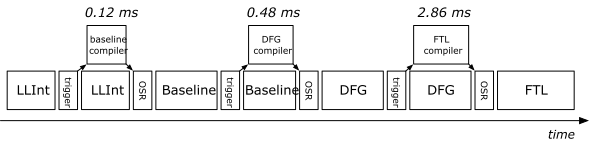
\includegraphics[width=.9\textwidth]{graphics/javascriptcore.png}
    \caption[JavaScriptCore loop]{\label{fig:JavaScriptcore}Voorbeeld tijdslijn van een simpele loop uitgevoerd in JavaScriptCore ~\autocite{Pizlo2020}}
\end{figure}

\subsection{Zig}
Een andere manier hoe Bun performanter probeert te zijn is door te kiezen voor de imperatieve, statisch getypeerde programmeertaal Zig. 
In een interview met ~\textcite{Motroc2017} legt de oprichter van Zig, Andrew Kelley, uit dat Zig bedoeld is als opvolger van de programmeertaal C.
Zo probeert hij met Zig het mogelijk te maken hoogperformante en onderhoudbare software te ontwikkelen 
zonder de moeilijkheden die voorkomen in andere programmeertalen zoals C, de programmeertaal gebruikt door Node.js.
Daarnaast is er nog altijd enige vorm van compatibiliteit met C, 
zo kunnen bijvoorbeeld functies geëxporteerd  worden zodat ze kunnen worden opgeroepen uit C.

\subsection{Test runner}
Bun bevat een ingebouwde test runner die volgens ~\textcite{McDonnel2023} 10 tot 30 keer sneller werkt als jest, een ander test-framework dat vaak wordt gebruikt in Node.js projecten.
De test runner ondersteunt zowel JavaScript als TypeScript. Hierbij is het ook mogelijk om mocks gebruiken.
Dit zijn valse objecten die de achterliggende functionaliteit simuleren om zo externe afhankelijkheden zelf te controleren.
In het codefragment ~\ref{list:testbun} wordt een voorbeeld van een test binnen bun weergegeven.
\begin{listing}[H]
    \centering
    \begin{minted}[bgcolor=bg,
        fontfamily=tt,
        linenos=true,
        numberblanklines=true,
        numbersep=5pt,
        gobble=0,
        framesep=2mm,
        tabsize=4,
        obeytabs=false,
        breaklines=true,
        mathescape=false
        samepage=false,
        showspaces=false,
        showtabs =false,
        texcl=false]{js}
import { expect, test } from "bun:test";

test("1 + 1", () => {
    expect(1 + 1).toBe(2);
});
        \end{minted}
        \caption[Bun test]{\label{list:testbun}Voorbeeld test binnen Bun ~\autocite{McDonnel2023}}
\end{listing}

\subsection{Package manager}
Net zoals Node.js bevat ook Bun een package manager. 
Deze is compatibel met Node.js waardoor dus ook een package.json gebruikt kan worden.
Onderzoek van ~\textcite{McDonnel2023} zou aantonen dat de package manager 
van Bun tot 25 keer sneller packages zou kunnen installeren tegenover Node.js.
Hierbij wordt tijdens het installeren van een package, 
deze gedownload in een globale package cache. Zo kan bij toekomstige installaties 
eerst de cache gecontroleerd om onnodige downloads te vermijden. Na de installatie zal Bun een binaire lockfile maken. 
Deze bevat zaken zoals de packages, de metadata van deze packages, versies etc. Door het binaire formaat kan er sneller gelezen worden dan bij JSON-gebaseerde lockfiles zoals in Node.js.
Daarnaast kan Bun, in tegenstelling tot npm, ook aan tree shaking doen waarbij ongebruikte code niet wordt meegenomen ~\autocite{Aghdasi2023}.


\subsection{Bundler}
Bun heeft een ingebouwde bundler die zowel via de commandolijn als binnen de code zelf kan worden aangeroepen. 
De bundler helpt op verschillende vlakken ~\autocite{McDonnel2023}:
\begin{itemize}
    \item De bundler helpt om het aantal HTTP verzoeken te verminderen door het kleiner aantal bestanden dat moet worden ingeladen.
    \item De bundler zal TypeScript en CSS modules omzetten naar gewone JavaScript en CSS. 
    \item Frameworks zijn afhankelijk van bundler plugins om algemene zaken te implementeren zoals de routering van bestandssystemen.
\end{itemize}
De bundler van Bun zou bovendien ook sneller zijn dan bestaande bundlers zoals Esbuild en Webpack.

\subsection{TypeScript ondersteuning}
Net zoals Deno ondersteunt Bun TypeScript als standaard. 
Zo zal de interne transpiler van Bun de TypeScript automatisch omzetten in JavaScript vóór de executie.
Hierbij kan ook gebruikgemaakt worden van een tsconfig.json bestand om de nodige configuratie in te stellen.
In figuur ~\ref{fig:nodevbun} wordt nog eens een visuele voorstelling getoond van de verschillen tussen Node.js en Bun

\begin{figure}[H]
    \centering
    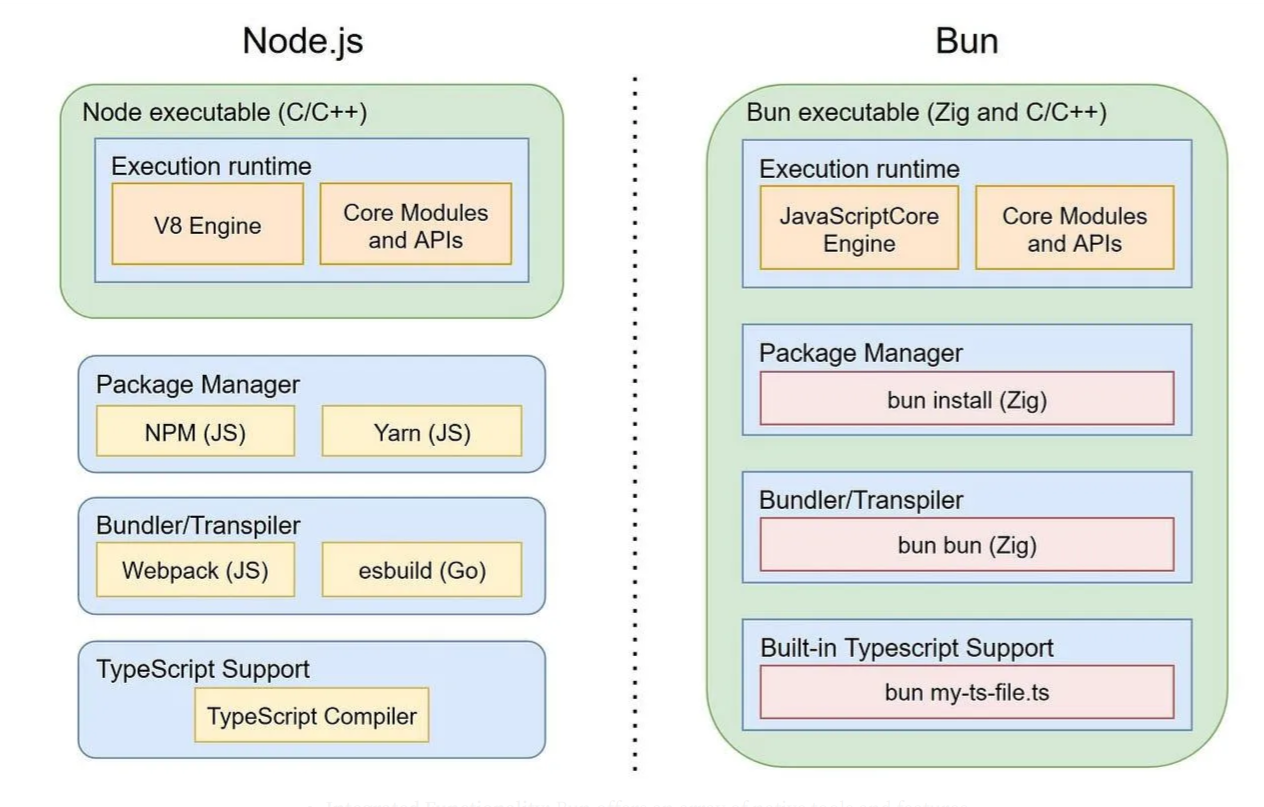
\includegraphics[width=.9\textwidth]{graphics/nodevbun.png}
    \caption[Verschillen Node.js en Bun]{\label{fig:nodevbun}Visuele voorstelling van de verschillen tussen Node.js en Bun ~\autocite{Aghdasi2023}}
\end{figure}

\section{Bun tegenover Node.js}
Doordat Bun redelijk nieuw is, zijn er nog maar weinig onderzoeken overgedaan. Eén van deze weinige
onderzoeken werd uitgevoerd door ~\textcite{Feroj2023}. 

In dit onderzoek werd de performantie tussen Node.js en Bun vergeleken op basis van het product kwaliteit model binnen ISO/IEC 25010.
Deze software kwaliteit standaard helpt volgens ~\textcite{Britton2021} te bepalen of de software van hoge kwaliteit is.
Deze bestaat concreet uit 8 product kwaliteit karakteristieken waarbij binnen het onderzoek gefocust werd op performantie efficiëntie.
Aan de hand performantie metrieken kan de software worden geëvalueerd. 
Hierbij verwijst performantie efficiëntie naar het aantal middelen die worden gebruikt.
Dit kan onderverdeeld worden in 3 zaken ~\autocite{Britton2021}:
\begin{itemize}
    \item Het tijdgedrag wat verwijst naar de respons- en verwerkingstijden alsook de doorvoersnelheden wanneer een systeem zijn functies uitvoert.
    \item Het gebruik van middelen dat wordt verbruikt tijdens de uitvoering.
    \item De capaciteit dat verwijst naar de limieten van het systeem.
\end{itemize}



In het onderzoek werd binnen de context van tijdgedrag gekeken naar de responstijd en uitvoeringstijd. 
Dit is de tijd die het systeem respectievelijk nodig heeft om te antwoorden op een gebeurtenis en de functie effectief uit te voeren.
Daarnaast werd ook gekeken naar het gebruik van middelen op vlak van geheugen.
Als laatste werd ook de capaciteit van het systeem bekeken door het gebruik van aparte scenario's met telkens een verschillend aantal connecties.
In het onderzoek werden 2 soort omgevingen gemaakt. Allereerst werd voor zowel Node.js als Bun een server gemaakt die netwerkverzoeken moet afhandelen.
Daarnaast werd ook getest hoe beide runtimes een alleenstaand script afhandelden.
Om de server te testen werd gebruikgemaakt van Bombardier. Dit is een HTTP benchmarking software ontwikkeld door ~\textcite{Fedoseev2023}.
\begin{listing}[H]
    \centering
    \begin{minted}[bgcolor=bg,
        fontfamily=tt,
        linenos=true,
        numberblanklines=true,
        numbersep=5pt,  
        gobble=0,
        framesep=2mm,
        tabsize=4,
        obeytabs=false,
        breaklines=true,
        mathescape=false
        samepage=false,
        showspaces=false,
        showtabs =false,
        texcl=false]{shell}
        > bombardier -c 125 -n 10000000 http://localhost:8080
        Bombarding http://localhost:8080 with 10000000 requests using 125 connections
         10000000 / 10000000 [============================================] 100.00% 37s Done!
        Statistics        Avg      Stdev        Max
          Reqs/sec    264560.00   10733.06     268434
          Latency      471.00us   522.34us    51.00ms
          HTTP codes:
            1xx - 0, 2xx - 10000000, 3xx - 0, 4xx - 0, 5xx - 0
            others - 0
          Throughput:   292.92MB/s
        \end{minted}
        \caption[Gebruik Bombardier]{Voorbeeld gebruik Bombardier \autocite{Fedoseev2023}}
\end{listing}
Hiernaast werd ook het ingebouwde time-commando gebruikt om het geheugengebruik tijdens zware belastingen te meten.
Bij de testen werd gewerkt met 3 aparte scenario's waarbij telkens 10 miljoen verzoeken werden verstuurd met eerst 10 gelijktijdige connecties, 
dan 100 gelijktijdige connecties en uiteindelijk 500 gelijktijdige connecties.
Hierbij kon de onderzoeker de performantie van de servers evalueren aan de hand van respons- en doorvoertijd. Aanvullend werden ook de geheugengebruik pieken bepaald.
Op vlak van geheugengebruik zat Bun consistent lager dan Node.js wat volgens de onderzoeker aantoont dat Bun een beter geheugenbeheer heeft. 
De onderzoeker merkt op dat de oorzaak hiervan ligt bij Bun's gebruik van de programmeertaal Zig. 
Ook op vlak van responstijd en doorvoertijd presteerde Bun beter dan Node.js in alle 3 scenario's.
De onderzoeker merkt hierbij op dat de reden hiervoor ligt bij Bun's beter geoptimaliseerde code.


Voor de andere test werd de executie tijd gemeten bij het berekenen van het veertigste Fibonacci nummer in zowel Node.js als Bun. 
Dit werd gedaan met behulp van de benchmarking software Hyperfine ontwikkeld door ~\textcite{Pompeii2024}. 
Het script werd 10 keer uitgevoerd waarbij de gemiddelde tijd werd genomen.
\begin{listing}[H]
    \centering
    \begin{minted}[bgcolor=bg,
        fontfamily=tt,
        linenos=true,
        numberblanklines=true,
        numbersep=5pt,  
        gobble=0,
        framesep=2mm,
        tabsize=4,
        obeytabs=false,
        breaklines=true,
        mathescape=false
        samepage=false,
        showspaces=false,
        showtabs =false,
        texcl=false]{shell-session}
        > hyperfine 'sleep 0.3'
        \end{minted}
        \caption[Gebruik Hyperfine]{Voorbeeld gebruik Hyperfine commando \autocite{Pompeii2024}}
\end{listing}
Ook bij deze test presteerde Bun beter op vlak van executie tijd wat volgens de onderzoeker aantoont dat Bun effectiever is in het voltooien van computationele taken.
De resultaten tonen aan dat 
Bun algemeen beter presteert in alle gemeten performantie aspecten.
De onderzoeker merkt echter ook op dat de keuze van een runtime niet alleen kan bepaald worden op basis van 
performantie. Andere factoren, die hier niet getest zijn, zoals beveiliging, stabiliteit en onderhoudbaarheid dragen ook bij tot de keuze. 
Ook waren de geteste programma's redelijk simpel waardoor de resultaten mogelijks niet accuraat zijn voor complexere omgevingen. 
Verder onderzoek zou volgens de onderzoeker ook baat hebben om rekening te houden met verschillende omstandigheden, zoals CPU-gebonden
en I/O-gebonden processen, en andere performantie factoren.

\section{Andere gebruikte technologieën}
\subsection{Docker}
Voor omgevingen op te zetten wordt vaak een vorm van automatisatie gebruikt. 
Hierdoor wordt repliceerbaarheid van de omgeving bereikt. Een manier om dit te doen is met behulp van de tool Docker.
Deze tool laat containerisatie van een applicatie toe samen met de bijhorende configuratie \autocite{Ibrahim2021}.
Hierbij wordt een applicatie gedraaid in een container waarbij het besturingssysteem van de machine zelf wordt gebruikt \autocite{Boettiger2015}.
Als basis wordt een Docker image gebruikt. Dit is een binaire image waarin alle software al geïnstalleerd, geconfigureerd en getest is \autocite{Boettiger2015}.
Zo bestaan er voor zowel Node.js, Deno als Bun Docker images die kunnen gebruikt worden om de respectievelijke omgeving te installeren in de container.
Via een Dockerfile kan dan verder gebouwd worden op deze images om zo andere zaken toe te voegen en een nieuwe zelfgemaakte image te bekomen \autocite{Boettiger2015}.
Een visuele voorstelling van dit proces is te vinden in figuur ~\ref{fig:dockerproces}.
Veel applicaties bestaan uit meerdere zaken zoals een databank, server etc. 
Met behulp van Docker compose kunnen deze complexe applicaties worden samengesteld. 
Hierbij worden de verschillende componenten beschreven in een Docker Compose bestand waarbij specifiek hun
respectievelijke image en configuratie omschreven wordt \autocite{Ibrahim2021}.
\begin{figure}[H]
    \centering
    \includegraphics[width=.9\textwidth]{graphics/docker_proces.png}
    \caption[Docker proces]{\label{fig:dockerproces}Visuele voorstelling van het Docker proces ~\autocite{Ibrahim2021}}
\end{figure}

\subsection{ORM}
Binnen een applicatie wordt persistentie bereikt door gebruik te maken van een achterliggende database. 
Er zijn veel manieren om deze persistentie af te handelen in een applicatie.
Een bekende en makkelijke manier is door het gebruiken van een Object Relational Mapper (ORM).
Hierbij wordt persistentie bereikt door de objecten binnen de applicatie te koppelen aan tabellen in de databank \autocite{Lorenz2017}.
De ORM zal deze koppeling afhandelen en zo een abstractie creëren die de technische details van de mappingimplementatie verbergt \autocite{Lorenz2017}.
